% !TEX root = ./document.tex

\documentclass[a4paper, spanish]{article}

\usepackage{mystyle}
\usepackage{myvars}

\begin{document}

  \maketitle
  \begin{itemize}
    \item \textbf{Enunciado:} Llevar a cabo un estudio de simulación para aproximar la potencia, en la alternativa $t(2)$ (\emph{t de student con $2$ grados de libertad}), de los tests de nivel $\alpha = 0.05$ de \emph{Lilliefors}, \emph{Cramer-Von-Mises}, \emph{Anderson-Darling} y \emph{Shapiro-Francia}, para contrastar la hipótesis nula de normalidad, basados en muestras de tamaños $n \in \{10, 30, 60, 100, 150, 300, 500\}$. Hacer una representación gráfica (potencia frente a tamaño muestral) que resuma los resultados obtenidos, asignando colores diferentes a cada test.
  \end{itemize}

  \section{Introducción}

    \paragraph{}
    Para el contraste de la hipótesis de normalidad se han desarrollado una grán cantidad de métodos y técnicas que tratan de responder a la pregunta sobre si los datos observados en una determinada muestra pueden asumirse normales, o por contra, siguen una distribución diferente.


    \begin{equation*}
    \label{eq:test}
      \begin{split}
        H_0&: F \equiv Normal(\mu, \sigma^2) \\
        H_1&: F \not\equiv Normal(\mu, \sigma^2)
      \end{split}
    \end{equation*}

    \paragraph{}
    Para ello, se puede definir un test de \emph{bondad de ajuste} donde la hipótesis nula indica que la distribución $F$ de los datos observados es Normal, frente a la alternativa de que no lo sea. Dicho contraste se indica en la \autoref{eq:test}. Nótese que en este caso se ha llevado a cabo de manera compuesta (donde los parámetros de localización y escala son libres). Normalmente, cuando un contraste se define de esta manera, los parámetros $\mu$ y $\sigma ^ 2$ son estimados a partir de los datos observados. Es en estos casos donde cobran importancia los test que se describen a continuación.

    \paragraph{}
    En este caso, vamos a comparar $4$ tests de normalidad, los cuales describiremos a continuación: \emph{Lilliefors}, \emph{Cramer-Von-Mises}, \emph{Anderson-Darling} y \emph{Shapiro-Francia}. Posteriormente en la \autoref{sec:simulation} se describe la metodología llevada a cabo para la estimación de la potencia $\pi$ de los distintos tests. Finalmente, en la \autoref{sec:results} se muestran los resultados obtenidos.

    \paragraph{Lilliefors}
    El test de bondad de ajuste de \emph{Lilliefors} consiste en una variación del test de \emph{Kolmogorov-Smirnov}, que estima los parámetros de localilización y dispersión de la distribución normal a partir de los correpondientes valores muestrales $\overline{x}$ y $s^2$, permitiendo que la hipótesis nula sea compuesta.

    \begin{equation}
    \label{eq:test_lilliefors}
      \widehat{D}_n = sup_x \mid \widehat{F}_n(x) - F_0(x) \mid
    \end{equation}

    \paragraph{}
    Por lo tanto, el estadístico test se define en la \autoref{eq:test_lilliefors}, donde $\widehat{F}_n(x)$ es la función de distribución empírica y $F_0(x)$ la de una distribución $Normal(\overline{x}, s^2)$. En este caso, se utilizan unos valores críticos menos restrictivos obtenidos por simulación montecarlo, lo cual hace que el test sea menos conservador que el original de \emph{Kolmogorov-Smirnov}. El test rechaza la hipótesis nula para valores grandes del estadístico $\widehat{D}_n$.

    \paragraph{Cramer-Von-Mises}
    El test de bondad de ajuste de ajuste de \emph{Cramer-Von-Mises} está basado en el estadístico descrito en la \autoref{eq:test_cramervonmises}. Rechaza la hipótesis nula para valores grandes del estadístico $\widehat{W}^2_n$ y es más potente que el de \emph{Lilliefors}.

    \begin{equation}
    \label{eq:test_cramervonmises}
      \widehat{W}^2_n = n \int_{-\infty}^{\infty} \left(\widehat{F}_n(x) - F_0(x) \right)^2 d F_0(x)
    \end{equation}

    \paragraph{Anderson-Darling}
    El test de bondad de ajuste de ajuste de \emph{Cramer-Von-Mises} está basado en el estadístico descrito en la \autoref{eq:test_andersondarling}. Rechaza la hipótesis nula para valores grandes del estadístico $\widehat{W}^2_n$ y es muy similar en potencia al de \emph{Cramer-Von-Mises}.

    \begin{equation}
    \label{eq:test_andersondarling}
      \widehat{W}^2_n = n \int_{-\infty}^{\infty} \frac{\left(\widehat{F}_n(x) - F_0(x) \right)^2}{ F_0(x) (1 - F_0(x))} d F_0(x)
    \end{equation}

    \paragraph{Shapiro-Francia}
    Este test de bondad de ajuste se basa en una aproximación (más simple computacionalmente) del test de \emph{Shapiro-Wilk}, basada en la correlación al cuadrado entre los valores ordenados de la muestra y los esperados de una distribución $Normal(\overline{x}, s^2)$. Dado que el estadístico consiste en una correlación, estará entre $0$ y $1$, reschazando la hipótesis nula para valores próximos a $0$.

  \section{Simulación}
  \label{sec:simulation}

    \paragraph{}
    En este trabajo se ha comparado la potencia de los tests no paramétricos para la hipótesis de normalidad, frente a la alternativa, siendo esta una distribución \emph{t de student} con $2$ grados de libertad. Esto se va a llevar a cabo para distintos tamaños muestrales $n \in \{10, 30, 60, 100, 150, 300, 500\}$. En general, la potencia de un test se define como la capacidad para rechazar la hipótesis nula, cuando esta realmente es falsa. Mas matemáticamente esto es $\pi = P\left(\text{rechazar }H_{0} \mid H_{1} \text{ sea verdadero}\right)$.

    \paragraph{}
    A pesar de que para algunos constrastes de hipótesis se puede calcular analíticamente una expresión que permite expresear la potencia de un test fijando el tamaño muestral $n$ y el nivel de significancia $\alpha$, en general esto no es posible. Sin embargo, esto puede ser calculado mediante métodos de simulación conocemos la distribución de los datos en la hipótesis alternativa (y por tanto podemos generar observaciones procedentes de esta).

    \paragraph{}
    Para la simulación se puede recurrir a distintas técnicas, entre las que se encuentra el método de la función de distribución inversa. Este método consiste en calcular la función inversa de la función de distribución de la distribución que se pretende simular. Esto es $F^{-1}(x)$ y a partir de esta función, transformar valores simulados de una distribución $U \sim Uniforme(0,1)$ (que pueden obtenerse de manera sencilla con un ordenador). De esta manera se consiguen observaciones pertenecientes a la distribución $F$. Esto se debe a la propiedad que indica que $F^{-1}(U) \equiv F$, lo cual es cierto por el método jacobiano de transformación de variables.

    \paragraph{}
    Entonces, una vez se tiene una muestra de variables independientes de la distribución en la alternativa, es trivial calcular la potencia del test. Esto puede llevarse a cabo promediando el número de veces que la hipótesis nula $H_0$ es rechazada, que converge en probabilidad a la potencia del test.


    \paragraph{}
    En el \autoref{code:r} se indican las sentencias necesarias para realizar dicha simulación utilizando el lenguaje \texttt{R}.

    \begin{listing}[htb!]
      \centering
      \inputminted{R}{./normality-testing.r}
      \caption{Potencia de los tests de normalidad utilizando como alternativa una distirbución \emph{t de student} con $2$ grados de libertad.}
      \label{code:r}
    \end{listing}

  \section{Resultados}
  \label{sec:results}

    \paragraph{}
    La simulación se ha llevado a cabo mediante la generación de $1000$ para cada aproximación. De esta manera se han generado los resultados que se muestran en la \autoref{table:results}, que se han representado de manera gráfica en la \autoref{fig:results}.

    \begin{table}[htb!]
      \centering
      \begin{tabular}{|r||l|l|l|l|}
          \hline
          $n$ & \emph{Lilliefors} & \emph{Cramer-Von-Mises} & \emph{Anderson-Darling} & \emph{Shapiro-Francia}
          \csvreader[head to column names]{normality-testing.csv}{}
          {\\\hline\n & \Lilliefors & \CramerVonMises & \AndersonDarling & \ShapiroFrancia}
          \\\hline
      \end{tabular}
      \caption{Resultados de la simulación.}
      \label{table:results}
    \end{table}

    \paragraph{}
    En cuanto a la interpretación de los resultados, se puede apreciar que conforme el tamaño de muestra $n$ aumenta, la potencia del test $\pi$ tiene hacia $1$. En este caso, cuando la muestra supera las $n = 150$ observaciones, la potencia del test de normalidad es prácticamente $1$. Nótese que este valor depende de la distribución en la alternativa, que cuanto más similar sea a la distribución normal, más número de observaciones será necesario utilizar para que la potencia del test sea razonable.

    \paragraph{}
    En cuanto a la comparación entre los distintos métodos utilizados, parece que el test de \emph{Lilliefors} es el menos potente de los $4$ comparados, mientras que el de \emph{Shapiro-Francia} es el que más potencia presenta. Mientras que los métodos de \emph{Cramer-Von-Mises} y \emph{Anderson-Darling} se encuentran en la zona intermedia, proporcionando una potencia muy similar.

    \begin{figure}[htb!]
      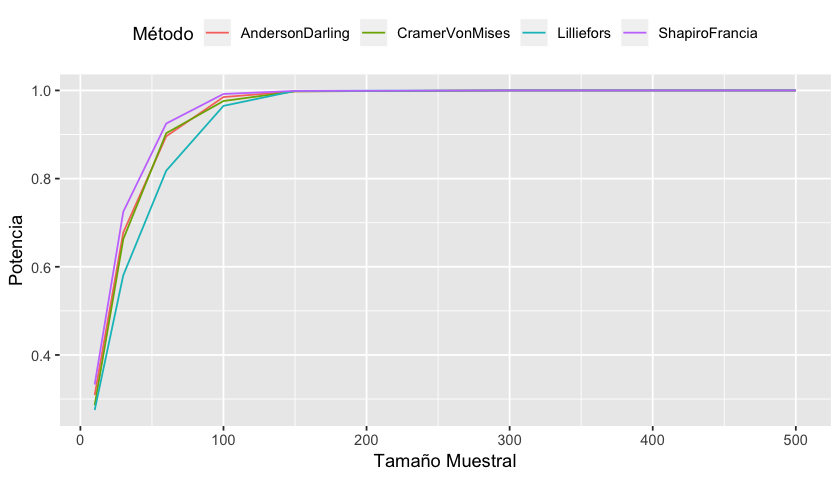
\includegraphics[width=\linewidth]{normality-testing}
      \caption{Resultados de la simulación.}
      \label{fig:results}
    \end{figure}


\end{document}
